\chapter{Situational \& Theoretical Analysis}\label{chap:situational_theoretical_analysis}

\section{The Thread Protocol}\label{sec:the_thread_protocol}
Thread is a low-power, wireless IoT protocol designed to provide secure, reliable, and scalable networking for connected devices. Developed by the Thread Group, which includes notable members such as Nest Labs (a subsidiary of Google), ARM, and Silicon Labs, Thread was introduced in 2014 to address the growing need for a standardized and efficient IoT networking solution. Built on open standards, Thread is an IPv6-based protocol that utilizes the IEEE 802.15.4 radio standard for communication, making it compatible with a wide range of existing devices and technologies \cite{Thread_Group_Fundamentals}.


\subsection{Architecture and Components}
Thread's architecture is based on a mesh topology, allowing devices to communicate directly with each other, bypassing the need for a central hub or router. This mesh design enhances network resilience, as devices can automatically re-route communication through alternative paths if a connection is lost. The key components of the Thread protocol include \cite{Thread_Group_Fundamentals}:

\begin{enumerate}
    \item \textbf{Border routers}: These devices serve as gateways between the Thread network and external IP networks, such as Wi-Fi or Ethernet networks. They manage network access, security, and routing of data between the Thread network and other networks.
    \item \textbf{Leader routers}: They play a vital role in managing the network by assigning addresses to devices, coordinating routing updates, and maintaining overall network stability.
    \item \textbf{Routers}: These devices are responsible for routing data within the Thread network. They can also act as parent devices to other devices within the network, providing connectivity to devices with limited routing capabilities.
    \item \textbf{End devices}: These devices communicate directly with their parent routers and are typically low-power devices, such as sensors or actuators. End devices do not participate in routing or network management.
    \item \textbf{Links}: Thread networks use links to establish connections between devices, allowing them to communicate and exchange data. Links are essential for maintaining the mesh topology of Thread networks.
\end{enumerate}

Figure \ref{fig:thread_topology} shows a visual representation of the basic Thread network topology, which includes all the listed components. By combining these components, the Thread network architecture provides a robust, scalable, and energy-efficient solution for IoT applications, including the MOOD-Sense project.

\begin{figure}[H]
    \centering
    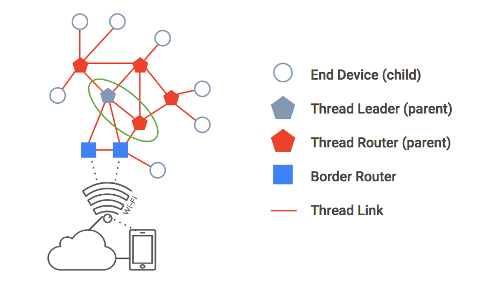
\includegraphics[width=0.5\textwidth]{images/situational_theoretical_analysis/thread_topology.png}
    \caption{Basic Thread network topology.}
    \label{fig:thread_topology}
\end{figure}


\subsection{Key Features and Advantages}

Considering the specific requirements of various IoT applications, including the MOOD-Sense project, the following features and advantages of Thread make it a suitable choice \cite{Thread_Group_Fundamentals}:

\begin{enumerate}
    \item \textbf{Low power consumption}: Thread's energy-efficient design aligns with the need for long battery life in devices that continuously monitor, collect, and transmit data in various IoT scenarios.
    \item \textbf{Scalability}: The mesh topology of Thread networks allows for the seamless addition of new devices, enabling IoT projects to adapt and expand as needed.
    \item \textbf{Security}: Thread's end-to-end encryption and secure commissioning processes ensure that communication between devices is protected, maintaining data privacy and security across diverse applications.
    \item \textbf{Robustness and reliability}: Thread's self-healing mesh network design ensures reliable and resilient communication, which is crucial for continuous monitoring and data collection in IoT applications.
    \item \textbf{Interoperability}: Thread's open standards ensure compatibility with a wide range of devices and technologies, allowing IoT projects to integrate various sensors, devices, and communication technologies within a single, unified network.
\end{enumerate}

Overall, the Thread protocol's features address the key question of its suitability for IoT applications in various contexts, including the MOOD-Sense project. Offering a secure, reliable, and energy-efficient networking solution, Thread meets the requirements for continuous monitoring, improved data collection, and seamless integration across industries.


\section{Power Optimization}\label{sec:power_optimization}

Optimizing power consumption in wireless IoT networks is a critical challenge, particularly for applications like the MOOD-Sense project, where devices are expected to operate for extended periods without frequent battery replacements or recharging. One effective approach to reduce power consumption is by minimizing transmission power while still maintaining reliable communication among devices, taking into account factors such as path loss and signal strength \cite{sheth2002implementation}. This section describes the implementation of transmission power control for Thread wireless networks, aiming to optimize the overall power consumption and ensure efficient and reliable communication among devices within the MOOD-Sense project context.

\subsection{Factors Influencing Transmission Power}

Parameters influencing transmission power in a Thread network are crucial for optimizing energy efficiency and network performance. By examining these factors, network designers can make informed decisions to achieve optimal performance under various conditions. A thorough understanding of these parameters is essential for implementing effective power management strategies and maintaining reliable communication within the network. Some of the factors include:

\subsubsection{Distance}

The distance between devices directly influences the transmission power, as a longer distance between devices typically results in higher path loss. Therefore, devices that are farther apart may require higher transmission power levels to maintain a stable connection. The Euclidean distance matrix calculates the distance between pairs of devices. The distance between devices $i$ and $j$ with coordinates $\left(x1,y1\right)$ and $\left(x2,y2\right)$ is calculated as follows:

\begin{equation}\label{eq:euclidean_distance}
    distance\left(i,j\right)=\sqrt{\left(x^2-x^1\right)^2+\left(y^2-y^1\right)^2}
\end{equation}

This calculation helps account for spatial constraints and device placements, ensuring Monte Carlo random input generation considers these factors for a more efficient and optimized Thread network \cite{dokmanic2015euclidean}.

\subsubsection{Received Signal Strength Indicator}

Received Signal Strength Indicator (RSSI) is a measurement of the power level of a received radio signal. It helps to determine the link quality between devices in a wireless network. A higher RSSI value indicates a stronger received signal, which may require lower transmission power to maintain reliable communication \cite{benkic2008rssi}. The RSSI calculation, including transmit and receive antenna gains, is:

\begin{equation}\label{eq:rssi}
    RSSI=P_t+G_t+G_r-L_p
\end{equation}

Where $RSSI$ represents the Received Signal Strength Indicator $\left(dBm\right)$, $P_t$ is the Transmission Power $\left(dBm\right)$, $G_t$ is the Transmit Antenna Gain $\left(dBi\right)$, $G_r$ is Receive Antenna Gain $\left(dBi\right)$, and $L_p$ is Path Loss $\left(dB\right)$ \cite{doi:10.1155/2014/371350}.

Thread devices typically have an RSSI sensitivity of -100 $dBm$. This formula applies to uplink and downlink connections, offering a more accurate signal strength representation and aiding in network performance optimization and energy consumption \cite{semiconductor_nrf52840_2018_1}.

\subsubsection{Antenna Gain}

The gain of the antennas used in the network can also affect the transmission power. A higher gain antenna can focus the radio signal more effectively, requiring less transmission power to achieve the same signal strength at the receiver \cite{wu2014study}.

\subsubsection{Path Loss}

Path loss refers to the attenuation of the radio signal as it propagates through the environment. It depends on factors such as the distance between transmitter and receiver, frequency, and environmental conditions. Path loss has a significant impact on the transmission power required to maintain reliable communication. This research analyzes three key path loss models and their applications in wireless communication systems.

\paragraph{Free-Space Propagation Model}

The free-space propagation model is used for predicting the received signal strength in line-of-sight (LOS) environments, where there are no obstacles between the transmitter and receiver. It is often adopted for satellite communication systems. The Friis equation \ref{eq:friis_equation} describes the received power at distance $d$, considering non-isotropic antennas with transmit gain $G_t$ and receive gain $G_r$ \cite{cho2010mimo}:

\begin{equation}\label{eq:friis_equation}
    P_r\left(d\right)=\frac{P_tG_tG_r\lambda^2}{\left(4\pi\right)^2d^2L}
\end{equation}

Where $P_t$ represents the transmit power $\left(w\right)$, $d$ is the distance between transmitter and receiver $\left(m\right)$, $\lambda$ is the wavelength of radiation $\left(m\right)$, $G_t$ is transmit gain $(dB)$, $G_r$ receive gain $(dB)$, and $L$ is the system loss factor independent of the propagation environment. The free-space path loss ${PL}_F\left(d\right)$ can be directly derived without any system loss from equation \ref{eq:friis_equation}:

\begin{equation}\label{eq:free_space_path_loss}
    PL_F\left(d\right)\left[dB\right]=10log\left(\frac{P_t}{P_r}\right)=-10log\left(\frac{G_tG_r\lambda^2}{\left(4\pi\right)^2d^2}\right)
\end{equation}

Without antenna gains (i.e., $G_t=G_r=1$), equation \ref{eq:free_space_path_loss} is reduced to:

\begin{equation}\label{eq:free_space_path_loss_no_antenna_gain}
    PL_F\left(d\right)\left[dB\right]=10log\left(\frac{P_t}{P_r}\right)=20log\left(\frac{4\pi d}{\lambda}\right)
\end{equation}

\paragraph{Log-Distance Path Loss Model}
The log-distance path loss model is a more generalized approach, accounting for the varying path loss exponent $n$ depending on the environment. The path loss at distance $d$ is given by equation \ref{eq:log_distance_path_loss}, where $d_0$ is the reference distance at which the path loss inherits the characteristics of free-space loss \cite{cho2010mimo}:

\begin{equation}\label{eq:log_distance_path_loss}
    PL_{LD}\left(d\right)\left[dB\right]=PL_F\left(d_0\right)+10nlog\left(\frac{d}{d_0}\right)
\end{equation}

Where $d_0$ is a reference distance and $n$ corresponds to free space which tends to change as shown in the following table.

\begin{longtable}{>{\hspace{0pt}}m{0.462\linewidth}>{\hspace{0pt}}m{0.467\linewidth}}
    \label{tab:path_loss_exponent}\\
    \caption{Path loss exponent for different environments.}\\
    \hline\hline
    Environment                   & Path Loss Exponent $(n)$  \endfirsthead
    \hline
    Free space                    & 2                         \\
    Urban area cellular radio     & 2.7 - 3.5                 \\
    Shadowed urban cellular radio & 3 - 5                     \\
    In building line-of-sight     & 1.6 - 1.8                 \\
    Obstructed in building        & 4 - 6                     \\
    Obstructed in factories       & 2 - 3                     \\
    \hline\hline
    \end{longtable}

The path loss exponent $\left(n\right)$ varies based on the environment, as shown in table \ref{tab:path_loss_exponent}, and helps to adjust the log-distance path loss model for more accurate predictions. Lower values represent environments with fewer obstructions, such as free space, while higher values indicate more complex environments with buildings or other obstacles.

\paragraph{Log-Normal Shadowing Model}

The log-normal shadowing model considers the random nature of shadowing effects, making it more suitable for realistic situations. The model is given by equation \ref{eq:log_normal_shadowing_model}, where $X_\sigma$ is a Gaussian random variable with a zero mean and a standard deviation of $\sigma$:

\begin{equation}\label{eq:log_normal_shadowing_model}
    PL\left(d\right)\left[dB\right]=\overline{PL}\left(d\right)+X_\sigma=PL_F\left(d_0\right)+10nlog\left(\frac{d}{d_0}\right)+X_\sigma
\end{equation}

In other words, this particular model allows the receiver at the same distance $d$ to have a different path loss, which varies with the random shadowing effect $X_\sigma$ \cite{cho2010mimo}.

\subsubsection{Device Types}

In a Thread network, devices can have different types and roles, such as routers, end devices, or border routers. These roles can impact the transmission power requirements, as routers may need to communicate with multiple neighboring devices, whereas end devices only need to communicate with their parent router \cite{Thread_Group_Fundamentals}.

\subsection{Algorithmic Approaches}

To optimize transmission power in a Thread network, algorithmic approaches can be employed. In this research, two algorithms are used to address transmission power optimization: the Monte Carlo Method (MCM) and the Genetic Algorithm (GA). The MCM focuses on selecting the right device types and configuring an optimal network based on the constraints and requirements of the MOOD-Sense project. The GA, on the other hand, takes the output from the MCM and optimizes the transmission power settings for each device, ensuring minimal energy consumption while maintaining network performance.

\subsubsection{Monte Carlo Method}

The Monte Carlo Method (MCM) is a statistical method that uses random sampling and repeated computation to obtain numerical results. In the context of transmission power optimization, MCM will be used to generate random sets of device types, positions, and transmission powers, evaluate their performance, and identify the most suitable configuration for the Thread network \cite{kroese2014monte}. The steps for implementing MCM in this research are as follows:

\begin{enumerate}
    \item Define the parameter space, including the range of values for each parameter involved in the network configuration.
    \item Generate a large number of random configurations within the parameter space.
    \item Evaluate the performance of each configuration using predefined constraints, such as types of devices.
    \item Identify the configuration that satisfies the constraints and use it as the initial configuration for the GA.
\end{enumerate}

\subsubsection{Genetic Algorithm}

The Genetic Anglrothm (GA) is an optimization technique inspired by the process of natural selection. It uses a population of possible solutions and evolves them over time using genetic operators, such as mutation and crossover. In this research, GA will be used to further refine the initial configuration obtained from MCM and find the optimal transmission power for each device in the Thread network \cite{lambora2019genetic}. The steps for implementing GA in this research are as follows:

\begin{enumerate}
    \item Initialize the population with the best configuration obtained from MCM.
    \item Evaluate the fitness of each individual in the population based on the predefined constraints.
    \item Select the fittest individuals for reproduction using selection techniques, such as tournament selection or roulette wheel selection.
    \item Apply genetic operators (crossover and mutation) to generate offspring from the selected parents.
    \item Replace the least fit individuals in the population with the offspring.
    \item Repeat steps 2 to 5 for a predefined number of generations or until a convergence criterion is met.
    \item Obtain the final optimal configuration from the fittest individual in the population.
\end{enumerate}

By combining MCM and GA, the proposed algorithmic approach efficiently explores the parameter space and identifies the optimal configuration that minimizes power consumption while maintaining network performance and reliability in the Thread network. Addressing the sub-research question 3, this research demonstrates the effectiveness of the combined approach in achieving the desired outcomes.

\subsection{Step-by-Step Guide for Power Optimization}

\begin{enumerate}
    \item \textbf{Identify the influencing factors and parameters}: Determine the parameters that impact transmission power, such as distance between devices, path loss, signal strength, interference, and device types.
    \item \textbf{Develop the algorithms}: Implement the MCM and GA algorithms to address power optimization in the Thread network, considering the constraints and requirements of the MOOD-Sense project.
    \item \textbf{Determine optimal device types and network configuration}: Use the MCM to identify the appropriate device types and optimal network configuration for the Thread network.
    \item \textbf{Optimize transmission power settings}: Apply the GA to optimize the transmission power settings for each device in the network, ensuring minimal energy consumption while maintaining reliable communication.
    \item \textbf{Evaluate network performance}: Assess the overall performance of the Thread network, ensuring that the optimized power settings do not compromise the network's reliability or efficiency.
    \item \textbf{Iterate and refine}: Continuously refine the algorithms and network configuration as necessary to maintain optimal power consumption and network performance.
\end{enumerate}

Through exploring the factors influencing transmission power and employing algorithmic approaches, this research seeks to provide a comprehensive understanding of power optimization in a Thread network and its implications on energy efficiency and network performance in the context of the MOOD-Sense project.


\section{Hardware Analysis}

In this research, several hardware components were employed to implement and optimize the Thread network for power efficiency. Each hardware piece played a crucial role in different stages of the project:

\subsection{nRF52840 Development Kit}

The nRF52840 Development Kit (DK) is a versatile single-board development kit for Bluetooth 5, Bluetooth mesh, Thread, Zigbee, 802.15.4, ANT, and 2.4 $GHz$ proprietary applications on the nRF52840 SoC. In this research, the nRF52840 DK was used to develop and test the Thread network, acting as routers and end devices in the network topology. The development kit enabled the research team to implement and evaluate the network performance and power consumption under different configurations \cite{Semiconductor_Nordic_Product_Brief_2018_2.0}.

\begin{figure}[H]
    \centering
    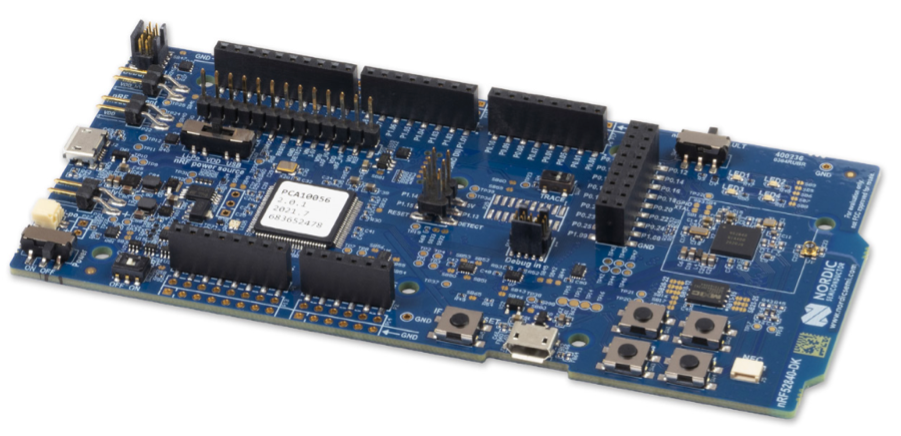
\includegraphics[width=0.3\textwidth]{images/situational_theoretical_analysis/nRF52840_DK.png}
    \caption{nRF52840 Development Kit.}
    \label{fig:nRF52840_DK}
\end{figure}

\subsection{nRF52840 Dongle}

The nRF52840 dongle is a small, low-cost USB device for the nRF Connect for Desktop PC tool. It supports Bluetooth 5, Bluetooth mesh, Thread, Zigbee, 802.15.4, ANT, and 2.4 GHz proprietary protocols. In the research, the dongle was used to extend the network by adding more nodes, facilitating the evaluation of scalability and network performance in larger network configurations sources \cite{Semiconductor_Nordic_Dongle_Brief_2018_2.0}.

\begin{figure}[H]
    \centering
    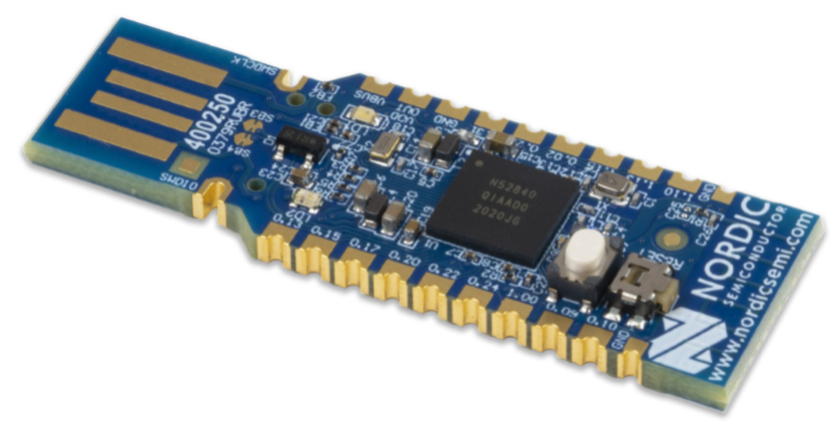
\includegraphics[width=0.3\textwidth]{images/situational_theoretical_analysis/nRF52840_Dongle.png}
    \caption{nRF52840 Dongle.}
    \label{fig:nRF52840_dongle}
\end{figure}

\subsection{Power Profiler Kit II}

The Power Profiler Kit (PPK) II is an easy-to-use tool for measuring and optimizing the power consumption of IoT devices. In this research, the Power Profiler Kit II was utilized to measure the power consumption of the nRF52840 DK devices in various network configurations, enabling the research to assess the energy efficiency of the network and identify areas for improvement \cite{Semiconductor_Nordic_PPK_II_2018_1.0}.

\begin{figure}[H]
    \centering
    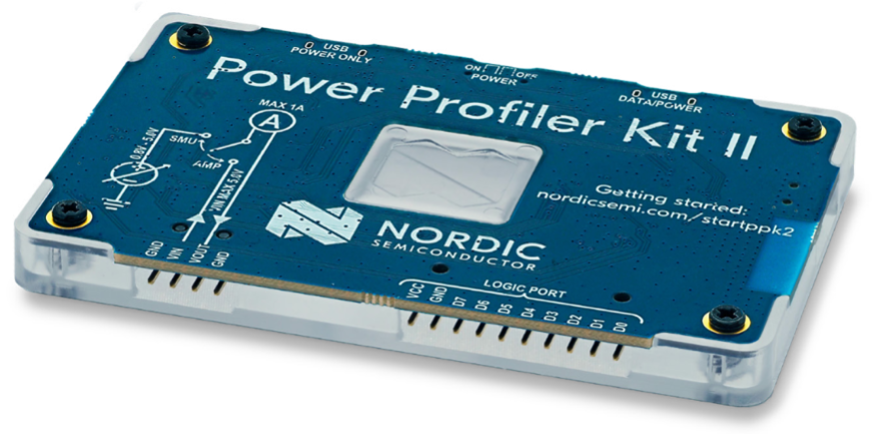
\includegraphics[width=0.3\textwidth]{images/situational_theoretical_analysis/nRF_Power_Profiler_Kit_II.png}
    \caption{Power Profiler Kit II.}
    \label{fig:nRF_Power_Profiler_Kit_II}
\end{figure}

\subsection{Raspberry Pi 4}

The Raspberry Pi 4 model B is a single-board computer used for various applications, including IoT development. In this research, the Raspberry Pi 4 served as a border router and provided an interface between the Thread network and external networks. The Raspberry Pi 4 allowed the research to evaluate the overall network performance and data exchange with external systems \cite{alm2019internet}.

\begin{figure}[H]
    \centering
    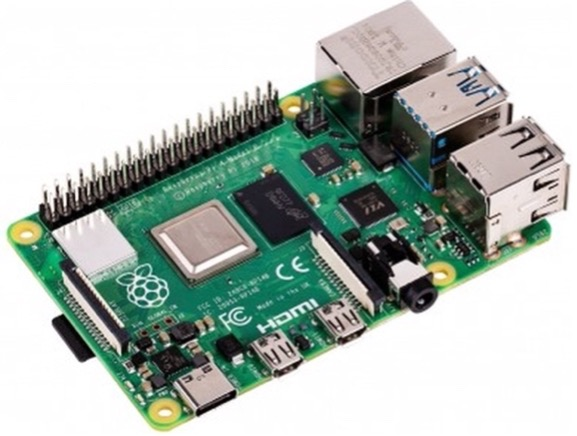
\includegraphics[width=0.3\textwidth]{images/situational_theoretical_analysis/Raspberry_Pi_4.jpg}
    \caption{Raspberry Pi 4 model B.}
    \label{fig:Raspberry_Pi_4}
\end{figure}

By understanding the roles of each hardware component in the research, it becomes evident how they collectively contributed to the successful implementation and optimization of the Thread network for power efficiency.

\subsection{Constraints and Limitations}

Using these hardware components poses certain constraints and limitations on the research, with some potential consequences:

\begin{enumerate}
    \item \textbf{Limited scalability}: The number of available nRF52840 DK and nRF52840 Dongle devices may limit the size of the network being optimized, potentially affecting the generalizability of the results. This limitation might make it challenging to extrapolate the findings to larger networks or different device types.
    \item \textbf{Hardware-specific performance}: The optimization results might be influenced by the specific hardware used, such as the nRF52840 DK and nRF52840 Dongle, and may not be directly applicable to other devices or platforms. As a consequence, further research and testing may be required to confirm the findings' applicability in different hardware contexts.
    \item \textbf{Measurement accuracy}: The accuracy of the Power Profiler Kit II may impact the precision of the power consumption measurements, potentially affecting the optimization results. This limitation could lead to underestimation or overestimation of energy savings, influencing the overall conclusions regarding the network's energy efficiency.
\end{enumerate}

These hardware-related challenges could influence the research outcomes, making it essential to be aware of the limitations and consider their potential impact on the findings when interpreting the results and applying them to real-world scenarios.

\subsection{Implications for Wireless Network Technology Development}

Taking into account the hardware constraints and limitations, the implications for wireless network technology development in the context of this research can be examined. The chosen hardware components, such as the nRF52840 DK, and nRF52840 Dongle directly impact the energy efficiency, performance, and scalability of the Thread network. Using these components enabled the investigation and optimization of power consumption and network performance. However, it is essential to acknowledge that hardware limitations might pose challenges when adapting the network to various IoT applications or scaling it to larger configurations. By addressing the sub-research question 4, this study highlights the importance of hardware selection and its implications for future wireless network technology development.

\section{Literature Research}\label{sec:literature_research}

Thread network power consumption research has been limited but offers promising results. One study by \textcite{semiconductor_battery_2021} demonstrates that the battery life of a Thread node is heavily dependent on the network configuration. For example, a node with an idle current of 3 $\mu A$ and a transmit current of 17 $mA$ can last up to 10 years in a network with a low data rate of 250 $kbps$ and a small number of packets per day. However, in a network with a high data rate of 1 $Mbps$ and many packets per day, the same node would only last for a few months. A white paper by \textcite{Thread_Low_Power_2018} provides noteworthy results on the power consumption and optimization of Thread networks, showing that the Thread protocol could achieve a standby power consumption of less than 3 $mW$, with typical transmit and receive power consumption ranging between 15 $mW$ and 20 $mW$. The study also demonstrated that devices on a Thread network could achieve up to 10 years of battery life when transmitting once per minute, making Thread a strong candidate for low-power IoT applications. Another research effort, conducted by \textcite{azoidou2017battery} analyzed the power consumption of Thread end devices, routers, and coordinators. The study demonstrated that enabling power management features could reduce power consumption by up to 70\% in sleep mode. Additionally, two power optimization techniques, dynamic power management and dynamic voltage and frequency scaling, were evaluated, with the latter having a greater impact, reducing consumption by up to 35\%. The research also emphasized that power consumption is influenced by transmission power level, data rate, and routing topology and suggested that implementing optimization techniques could reduce power consumption by up to 70\%.

In the paper by \textcite{sheth2002implementation} presents a practical implementation of transmit power control for 802.11b wireless networks. They focus on optimizing transmit power to reduce power consumption while maintaining correct reception of packets. The researchers achieved a maximum power savings of 25\%, including idling power, by implementing their adaptive transmit power control algorithm as a user-level application layer process. This work is relevant to power optimization strategies in IoT applications, such as Thread networks. \textcite{1576539} investigate the impact of transmission power on the throughput capacity of finite ad hoc wireless networks using a scheduling-based MAC protocol in their paper, such as TDMA. The authors demonstrate that by properly increasing the nodal transmit power level, the capacity of an ad hoc wireless network can be maximized, regardless of nodal distribution and traffic pattern. The primary finding is that higher transmission power contributes to increased combinatorial diversity, optimizing joint scheduling and routing schemes, which is valuable for the development of efficient IoT applications using protocols like Thread.

In the realm of algorithm optimization, the Monte Carlo method (MCM) is a robust, efficient, flexible, and scalable tool used across various fields, including science, finance, and engineering. Research by \textcite{kroese2014monte} emphasizes MCM's popularity and its applications in areas like industrial engineering, operations research, physical processes, random graphs, finance, biology, medicine, and computer science. The authors highlight MCM's simplicity, strength in randomness, and theoretical justification. On the other hand, Genetic Algorithm (GA) is a heuristic optimization algorithm that handles non-linear, non-convex, and intermittent problems. It is widely applied in various engineering and scientific applications. One study by \textcite{ferentinos2005energy} employs GA to optimize wireless sensor networks (WSNs) for precision agriculture applications. The research determines active sensors, cluster heads, and signal ranges while considering network connectivity, energy conservation, and application requirements. Results indicate that GA-generated designs outperform random deployments regarding connectivity and energy consumption. \textcite{norouzi2014genetic} explore the potential of GA in optimizing the operational stages of WSNs, discussing node placement, network coverage, clustering, data aggregation, and routing. Simulations demonstrate that GA-based approaches outperform existing protocols, suggesting that GA can optimize WSNs in military, medical, and commercial applications.

In summary, although the literature on Thread power optimization is limited, the results from existing studies suggest that the protocol has significant potential for reducing energy consumption in low-power wireless networking applications. More research is needed to fully understand and optimize the power consumption of Thread networks in large-scale deployments. Meanwhile, MCM and GA have significantly influenced quantitative problem-solving across numerous research fields, becoming indispensable tools for understanding complex systems and optimizing parameters in various applications. However, their computational complexity increases with the number of parameters, making it challenging to apply to large-scale problems.
